\title{Codebook}
\author{Jin, Lai, Lam from YZU}
\date{\today}
\documentclass[a4paper, landscape, 8pt]{article}
\usepackage{listings}
\usepackage{xcolor}
\usepackage{multicol}
\usepackage{inconsolata}
\usepackage{fancyhdr}
\usepackage{graphicx}
\usepackage[ruled, linesnumbered]{algorithm2e}
\usepackage[top=50pt, left=20pt, right=20pt, bottom=20pt]{geometry}

\SetKwRepeat{Do}{do}{while}

\pagestyle{fancy}
\fancyhf{}
\rhead{Page \thepage}
\lhead{Codebook}
\rfoot{}

\definecolor{codegreen}{rgb}{0,0.6,0}
\definecolor{codegray}{rgb}{0.5,0.5,0.5}
\definecolor{codepurple}{rgb}{0.58,0,0.82}
\definecolor{codekeyword}{RGB}{51,51,255}
\definecolor{backcolor}{rgb}{0.95,0.95,0.92}
 
\lstdefinestyle{mystyle}{
    backgroundcolor=\color{backcolor},   
    commentstyle=\color{codegreen},
    keywordstyle=\color{codekeyword},
    numberstyle=\tiny\color{codegray},
    stringstyle=\color{codepurple},
    basicstyle=\ttfamily,
    breakatwhitespace=false,         
    breaklines=true,                 
    captionpos=b,                    
    keepspaces=true,                 
    numbers=left,                    
    numbersep=1pt,                  
    showspaces=false,                
    showstringspaces=false,
    showtabs=false,                  
    tabsize=2
}

\lstdefinelanguage{vim}
{
  % list of keywords
  morekeywords={
  set, let
  map, nmap,
  filetype,
  on, off,
  autocmd,
  Plugin,
  call,
   },
morecomment=[l]{"}, % l is for line comment
morestring=[b]' % defines that strings are enclosed in double quotes
}
 
\lstset{style=mystyle}

\graphicspath{{image/}}

\begin{document}
\begin{multicols*}{3}
\maketitle
\tableofcontents

\section{Environment}
\subsection{.vimrc}
\lstinputlisting[language=vim]{code/.vimrc}
\subsection{compile}
\lstinputlisting[language=sh]{code/compile.sh}
\subsection{copy}
\lstinputlisting[language=sh]{code/copy.sh}
\subsection{template}
\lstinputlisting[language=c++]{code/template.cpp}

\section{Structure}
\lstinputlisting[language=c++]{code/Structure.cpp}

\section{Code Note}
\lstinputlisting[language=c++]{code/Code_Note.cpp}

\section{Algorithm Note}
\begin{algorithm}[H]
    \caption{ArticulationPoints($G$)}
    \ForEach{vertex $u \in G.V$}{
        $u.cut = \textbf{false}$
    }
    \ForEach{vertex $u \in G.V$}{
        \uIf{$u.\pi == $ NIL}{
            \uIf{$u.numChildren > 1$}{
                $u.cut = \textbf{true}$
            }
        }
        \Else{
            \ForEach{$v \in G.Adj[u]$}{
                \uIf{$v.\pi == u$}{
                    \uIf{$v.low >= u.d$}{
                        $u.cut = \textbf{true}$
                    }
                }
            }
        }
    }
\end{algorithm}

\begin{algorithm}[H]
    \caption{Biconnect($G$)}
    $time = time + 1$ \\
    $u.d = time$ \\
    $u.low = time$ \\
    \ForEach{$v \in G.Adj[u]$}{
        \uIf{$v.d == 0$}{
            $v.\pi = u$ \\
            $Push((u, v), S)$ \\
            $Biconnect(G, v)$ \\
            $u.low = min(u.low, v.low)$ \\
            \If{$v.low >= u.d$}{
                start new component \\
                \Do{$(x_1, x_2 != (u, v) and x_1.d >= v.d)$}{
                    $(x_1, x_2) = Pop(S)$ \\
                    put $(x_1, x_2)$ in current component 
                }
            }
        }
        \ElseIf{$v != u.\pi$}{
            $Push((u, v), S)$ \\
            $u.low = min(u.low, v.d)$
        }
    }
\end{algorithm}

\begin{algorithm}[H]
    \caption{Bridge($G, u$)}
    $time = time + 1$ \\
    $u.d = time$ \\
    $u.low = time$ \\
    \ForEach{$v \in G.Adj[u]$}{
        \uIf{$v.d == 0$}{
            $v.\pi = u$ \\ 
            $Bridge(G, v)$ \\
            $u.low = min(u.low, v.low)$ \\
            \If{$v.low > u.d$}{
                $\{u, v\}$ is a bridge
            }

        }
        \ElseIf{$v \neq u.\pi$}{
            $u.low = min(u.low, v.d)$
        }
    }
\end{algorithm}

\begin{algorithm}[H]
    \caption{TopologicalSort($G$)}
    \ForEach{vertex $u \in G.V$}{
        $u.color = \textmd{WHITE}$
    }
    \ForEach{vertex $u \in G.V$}{
        \If{$u.color = \textmd{WHITE}$}{
            $DFS_Visit(G, u)$
        }
    }
\end{algorithm}

\begin{algorithm}[H]
    \caption{DFS\_Visit($G, u$)}
    $u.color = \textmd{GRAY}$ \\
    \ForEach{$v \in G.Adj[u]$}{
        \If{$v.color == \textmd{WHITE}$}{
            $DFS\_Visit(G, u)$
        }
    }
    $u.color = \textmd{BLACK}$
    insert $u$ onto the front of a linked list
\end{algorithm}

\section{C++ Library}
\lstinputlisting[language=c++]{code/Library.cpp}

\section{Other Tool}
\subsection{gdb}
\lstinputlisting[]{code/gdb}
\subsection{vim}

\section{Note}
\subsection{Preparing}
\begin{lstlisting}[]
check keyboard
check mouse
check printer
check judge system
check response message
build environment(vim, g++, shell)
\end{lstlisting}
\subsection{Response Message}
\begin{lstlisting}[]
//for DOMjudge
CORRECT
COMPILER-ERROR
TIMELIMIT
RUN-ERROR
WRONG-ANSWER
\end{lstlisting}
\end{multicols*}

\section{Image Note}
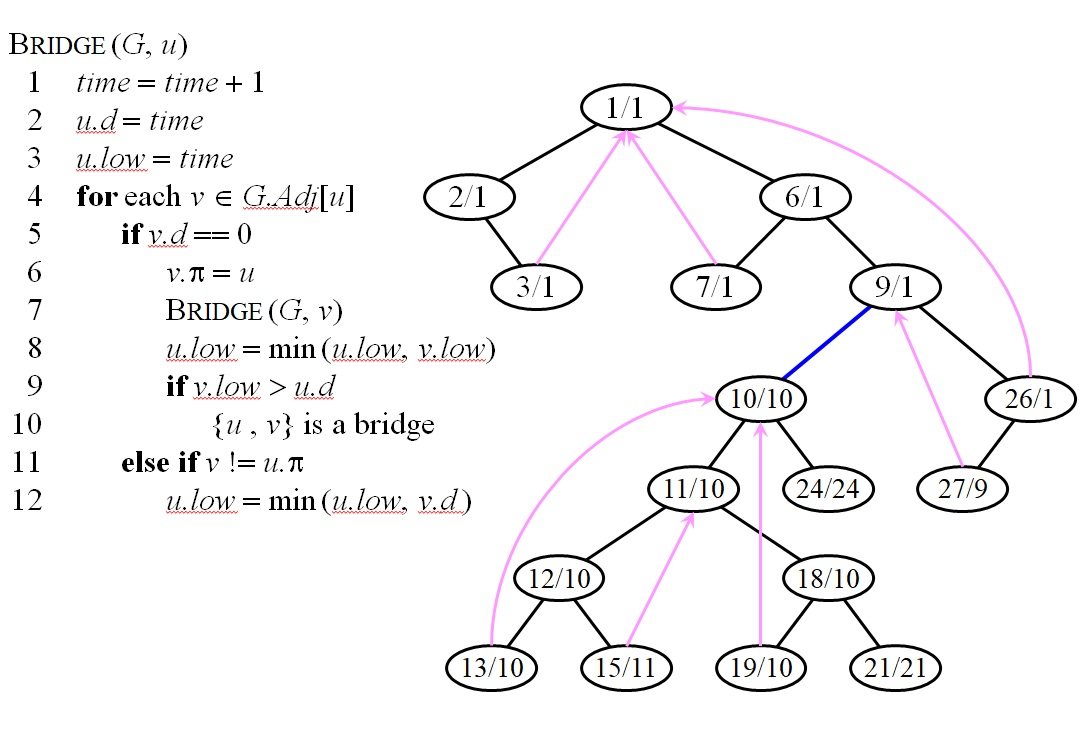
\includegraphics[]{Bridge} \clearpage
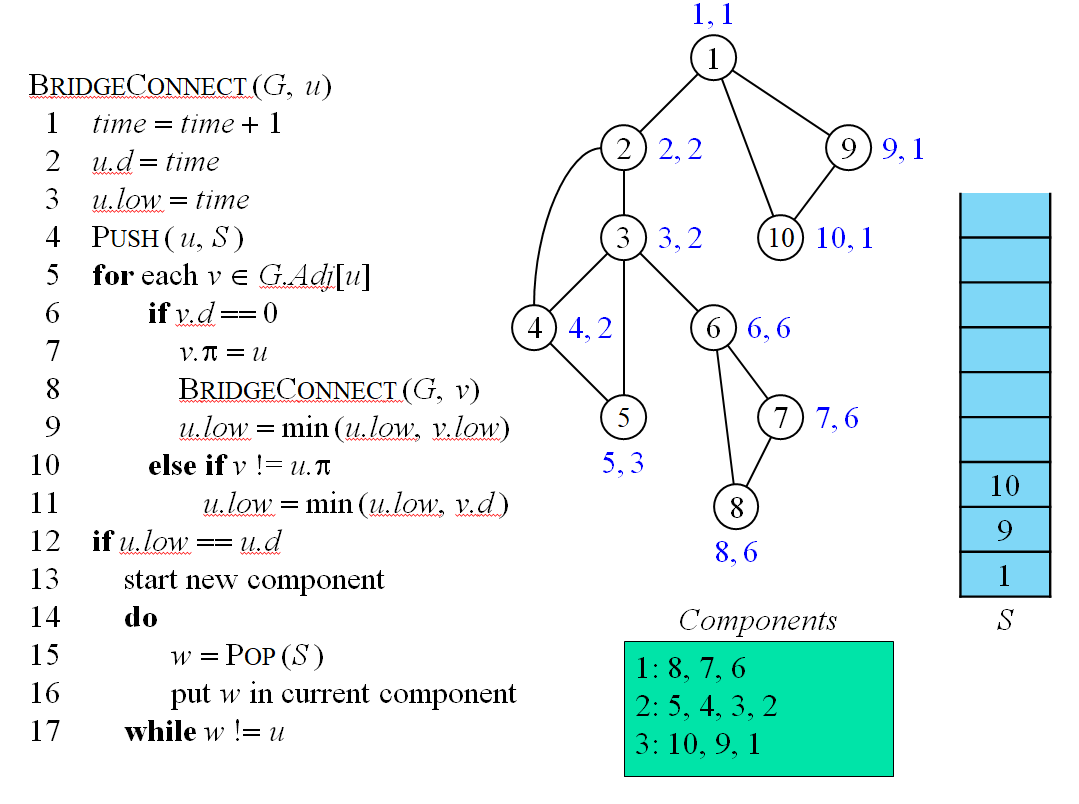
\includegraphics[]{BridgeConnect} \clearpage
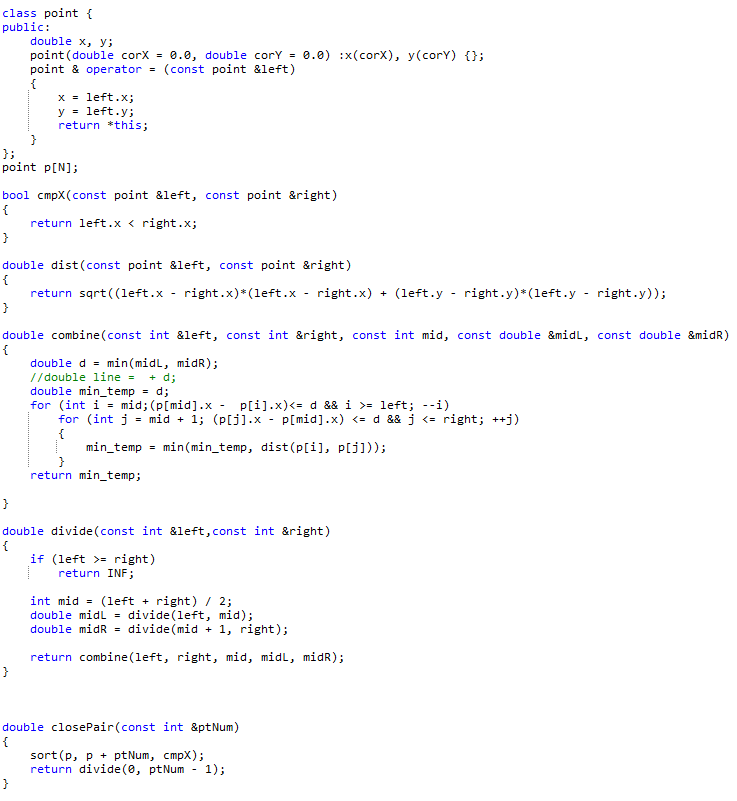
\includegraphics[]{ClosePair} \clearpage
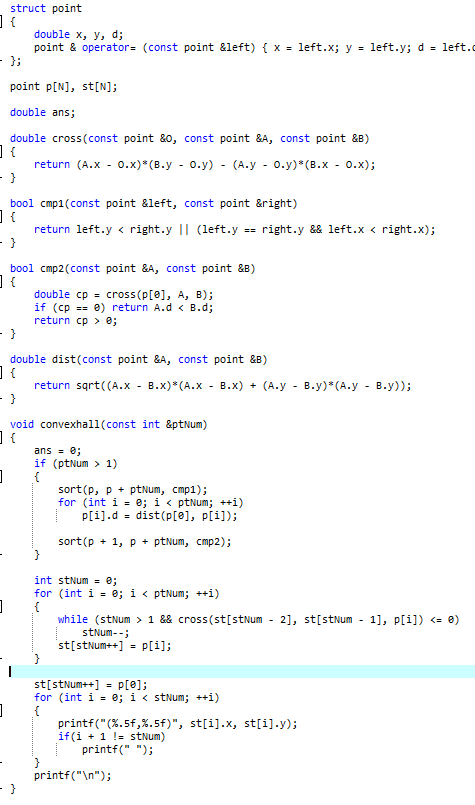
\includegraphics[]{ConvaxHall} \clearpage
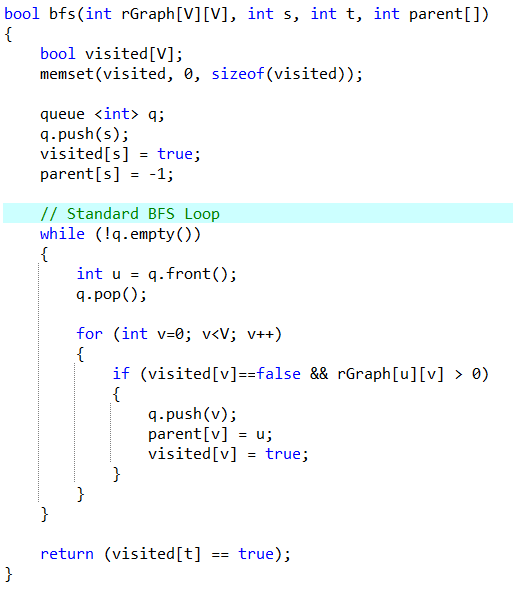
\includegraphics[]{MaximumFlow} \clearpage
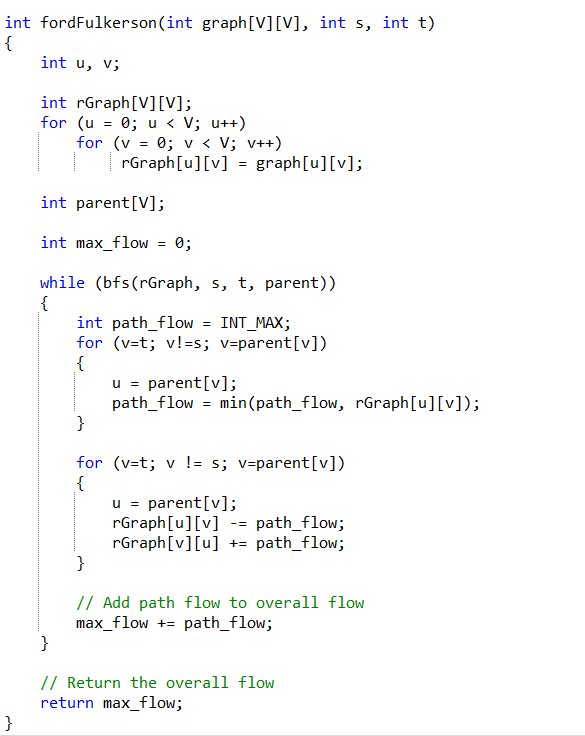
\includegraphics[]{MaximumFlow-2} \clearpage
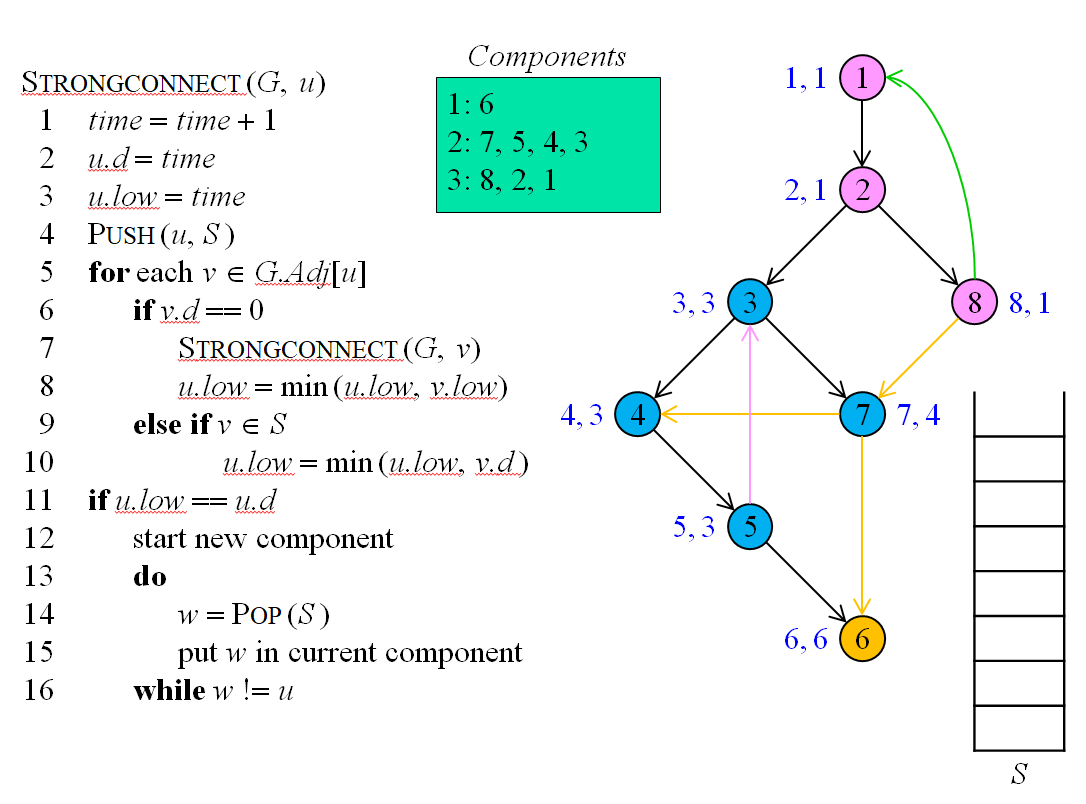
\includegraphics[]{StrongConnect} \clearpage

\end{document}